% Options for packages loaded elsewhere
\PassOptionsToPackage{unicode}{hyperref}
\PassOptionsToPackage{hyphens}{url}
%
\documentclass[
  5pt,
  ignorenonframetext,
]{beamer}
\usepackage{pgfpages}
\setbeamertemplate{caption}[numbered]
\setbeamertemplate{caption label separator}{: }
\setbeamercolor{caption name}{fg=normal text.fg}
\beamertemplatenavigationsymbolsempty
% Prevent slide breaks in the middle of a paragraph
\widowpenalties 1 10000
\raggedbottom
\setbeamertemplate{part page}{
  \centering
  \begin{beamercolorbox}[sep=16pt,center]{part title}
    \usebeamerfont{part title}\insertpart\par
  \end{beamercolorbox}
}
\setbeamertemplate{section page}{
  \centering
  \begin{beamercolorbox}[sep=12pt,center]{part title}
    \usebeamerfont{section title}\insertsection\par
  \end{beamercolorbox}
}
\setbeamertemplate{subsection page}{
  \centering
  \begin{beamercolorbox}[sep=8pt,center]{part title}
    \usebeamerfont{subsection title}\insertsubsection\par
  \end{beamercolorbox}
}
\AtBeginPart{
  \frame{\partpage}
}
\AtBeginSection{
  \ifbibliography
  \else
    \frame{\sectionpage}
  \fi
}
\AtBeginSubsection{
  \frame{\subsectionpage}
}
\usepackage{lmodern}
\usepackage{amssymb,amsmath}
\usepackage{ifxetex,ifluatex}
\ifnum 0\ifxetex 1\fi\ifluatex 1\fi=0 % if pdftex
  \usepackage[T1]{fontenc}
  \usepackage[utf8]{inputenc}
  \usepackage{textcomp} % provide euro and other symbols
\else % if luatex or xetex
  \usepackage{unicode-math}
  \defaultfontfeatures{Scale=MatchLowercase}
  \defaultfontfeatures[\rmfamily]{Ligatures=TeX,Scale=1}
\fi
\usetheme[]{Berlin}
\usecolortheme{beaver}
\usefonttheme{structurebold}
% Use upquote if available, for straight quotes in verbatim environments
\IfFileExists{upquote.sty}{\usepackage{upquote}}{}
\IfFileExists{microtype.sty}{% use microtype if available
  \usepackage[]{microtype}
  \UseMicrotypeSet[protrusion]{basicmath} % disable protrusion for tt fonts
}{}
\makeatletter
\@ifundefined{KOMAClassName}{% if non-KOMA class
  \IfFileExists{parskip.sty}{%
    \usepackage{parskip}
  }{% else
    \setlength{\parindent}{0pt}
    \setlength{\parskip}{6pt plus 2pt minus 1pt}}
}{% if KOMA class
  \KOMAoptions{parskip=half}}
\makeatother
\usepackage{xcolor}
\IfFileExists{xurl.sty}{\usepackage{xurl}}{} % add URL line breaks if available
\IfFileExists{bookmark.sty}{\usepackage{bookmark}}{\usepackage{hyperref}}
\hypersetup{
  pdftitle={Seminar},
  hidelinks,
  pdfcreator={LaTeX via pandoc}}
\urlstyle{same} % disable monospaced font for URLs
\newif\ifbibliography
\setlength{\emergencystretch}{3em} % prevent overfull lines
\providecommand{\tightlist}{%
  \setlength{\itemsep}{0pt}\setlength{\parskip}{0pt}}
\setcounter{secnumdepth}{-\maxdimen} % remove section numbering
\usepackage[orientation = landscape, size = custom, width = 16, height = 9, scale = 0.5]{beamerposter}
\setbeamertemplate{footline}[frame number]
\usefonttheme{serif}
% ## ---------------------------------------------------------------------- 
% \setbeamerfont{supervisor}{size = \scriptsize}
% \setbeamerfont{instructor}{size = \scriptsize}
% ## ---------------------------------------------------------------------- 
\defbeamertemplate{title page}{RunTemplate}
{
  \vfill
  % ## ---------------------------------------------------------------------- 
  \begin{beamercolorbox}[sep = 10pt, center]{titleGraph}
    \inserttitlegraphic
  \end{beamercolorbox}
  % ## ---------------------------------------------------------------------- 
  \begin{beamercolorbox}[sep = 8pt, center, rounded = true]{title}
    \usebeamerfont{title}\inserttitle\par
    \ifx\insertsubtitle\@empty
  \else
  {\usebeamerfont{subtitle}\usebeamercolor[fg]{subtitle}\insertsubtitle\par}
  \fi
  \end{beamercolorbox}
  % ## ---------------------------------------------------------------------- 
  \vskip0.4em
  % ## ---------------------------------------------------------------------- 
  \begin{beamercolorbox}[sep = 8pt, center]{author}
    \usebeamerfont{author}\insertauthor\par
  \end{beamercolorbox}
  % ## ---------------------------------------------------------------------- 
  % \begin{beamercolorbox}[sep = 5pt, center]{supervisor}
    % \usebeamerfont{supervisor}Supervisor: \supervisor
  % \end{beamercolorbox}
  % ## ---------------------------------------------------------------------- 
  % \begin{beamercolorbox}[sep = 5pt, center]{instructor}
    % \usebeamerfont{instructor}\instructor
  % \end{beamercolorbox}
  % ## ---------------------------------------------------------------------- 
  \begin{beamercolorbox}[sep = 8pt, center]{institute}
    \usebeamerfont{institute}\insertinstitute\par
  \end{beamercolorbox}
  % ## ---------------------------------------------------------------------- 
  \begin{beamercolorbox}[sep = 8pt, center]{date}
    \usebeamerfont{date}\insertdate\par
  \end{beamercolorbox}
  \vfill
}
\setbeamertemplate{title page}[RunTemplate]

\newenvironment{cols}[1][]{}{}

\newenvironment{col}[1]{\begin{minipage}{#1}\ignorespaces}{%
\end{minipage}
\ifhmode\unskip\fi
\aftergroup\useignorespacesandallpars}

\def\useignorespacesandallpars#1\ignorespaces\fi{%
#1\fi\ignorespacesandallpars}

\makeatletter
\def\ignorespacesandallpars{%
  \@ifnextchar\par
    {\expandafter\ignorespacesandallpars\@gobble}%
    {}%
}
\makeatother
\AtBeginEnvironment{longtable}{\tiny} \titlegraphic{\centering 
\includegraphics{./logo_lixiao.png}} \usepackage{caption} \captionsetup{font={tiny}} \usepackage{setspace} \setstretch{1.3} \linespread{1.3} \usepackage{xeCJK}

\title{Seminar}
\author{Lichuang Huang}
\date{2024-03-13}
\institute{Wie-Biotech}

\begin{document}
\frame{\titlepage}

\hypertarget{tasks-summary}{%
\section{Tasks summary}\label{tasks-summary}}

\begin{frame}{Overview 2024-01 \textasciitilde{} 2024-02}
\protect\hypertarget{overview-2024-01-2024-02}{}
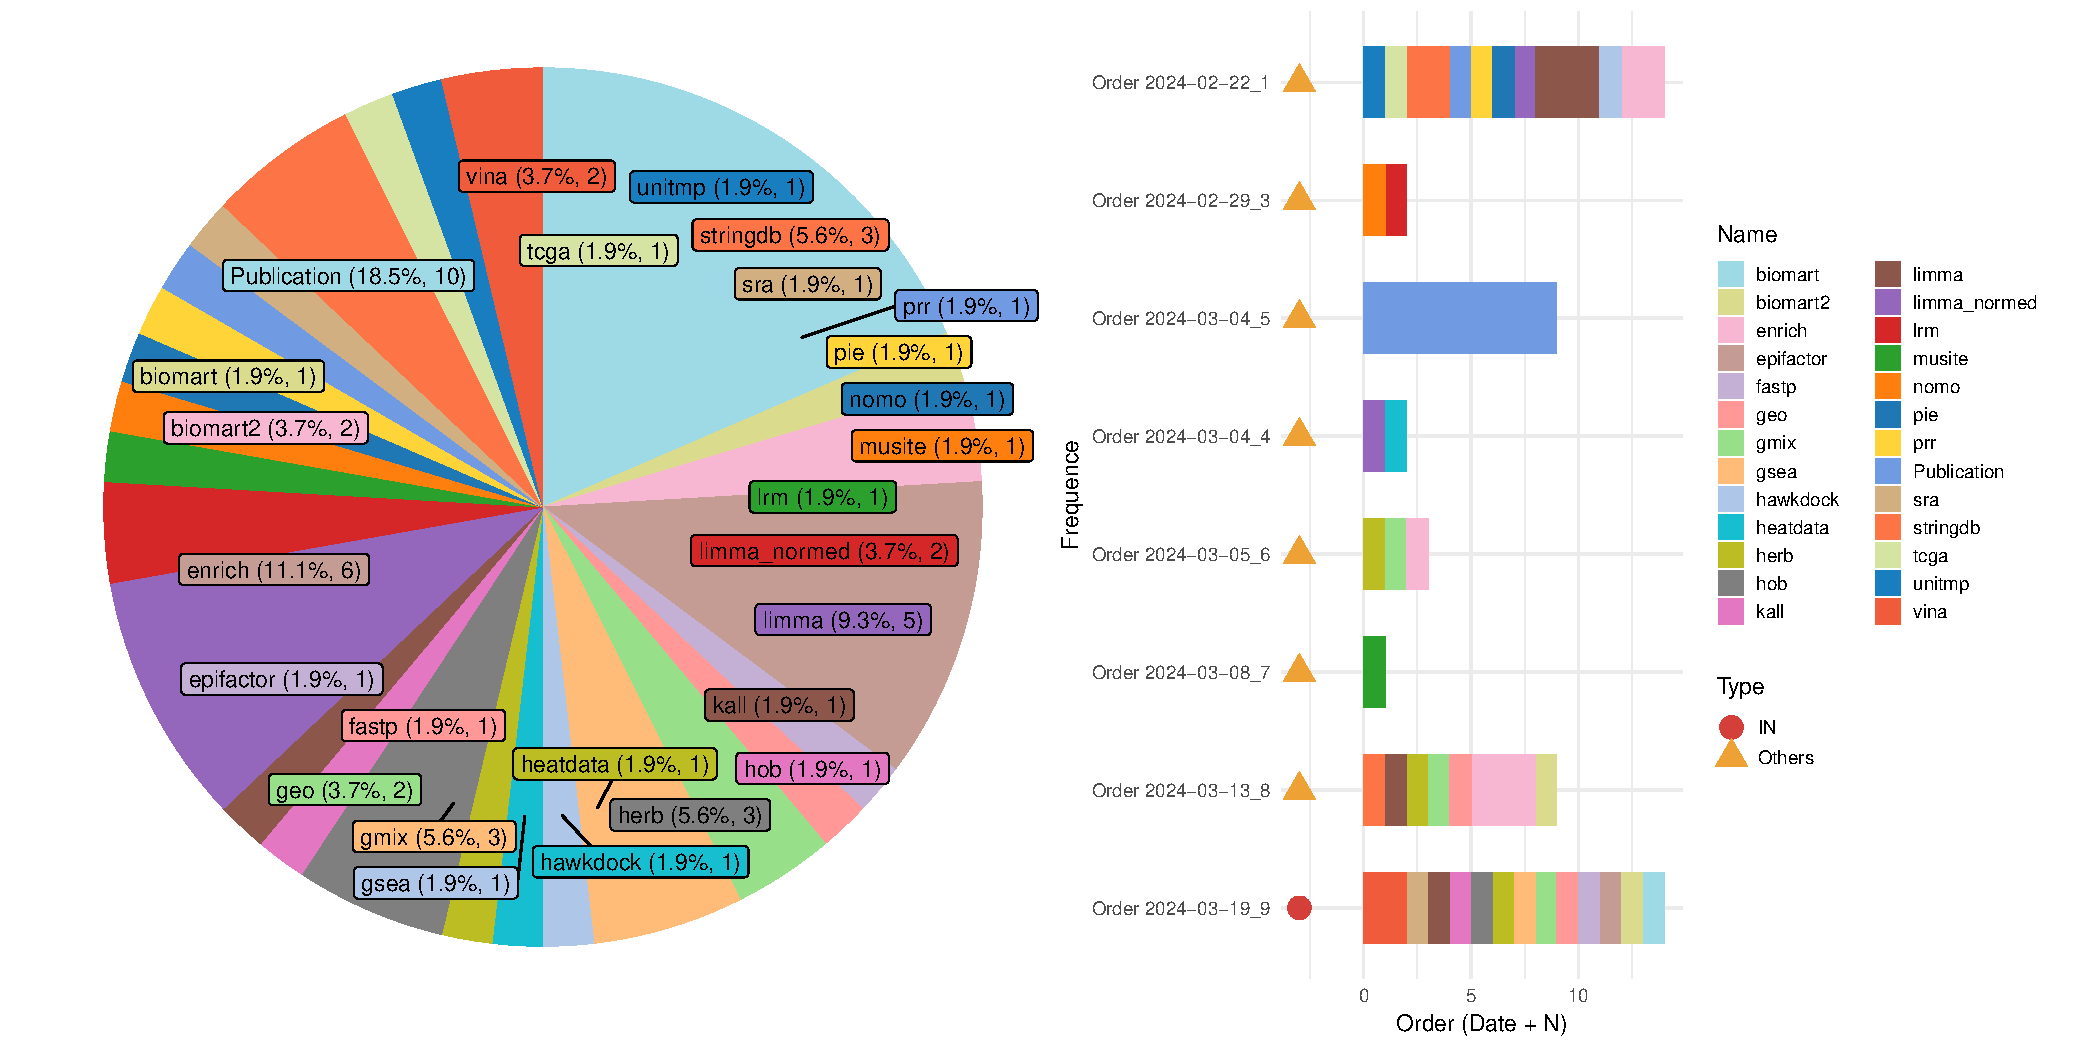
\includegraphics[height=65mm]{./figs/workflow2_01-02.pdf}
\end{frame}

\begin{frame}[fragile]{New Methods}
\protect\hypertarget{new-methods}{}
\begin{itemize}
\tightlist
\item
  gmix: \texttt{DisGeNet}, \texttt{GeneCards}, \texttt{PharmGKB}
\item
  lzerd: \texttt{LZerD} and \texttt{HawkDock} webservers,
  protein--protein docking
\item
  hob: Python, human oral bioavailability
\item
  plantdb: (crawler) The Database \texttt{PlantaeDB}
\item
  superpred: (crawler) drug-targets relationship prediction
  (SwissTargetPrediction)
\item
  ocr: Python, \texttt{doctr}
\item
  tfbs: (crawler) Transcription Factor Target Gene Database
\end{itemize}
\end{frame}

\begin{frame}[fragile]{New Methods}
\protect\hypertarget{new-methods-1}{}
\begin{itemize}
\tightlist
\item
  mpa: \texttt{MetaPhlAn}, microbial communities from metagenomic data
\item
  adcp: auto molecular docking (docking peptides)
\item
  nomo: logistic, nomogram
\item
  classyfire: systematic classification of chemical compounds
\item
  msconvert: file formats of MASS data
\item
  xcms: MASS data preprocessing
\end{itemize}
\end{frame}

\hypertarget{article-sharing}{%
\section{Article sharing}\label{article-sharing}}

\begin{frame}{Reconstruction of colon cancer microbiome}
\protect\hypertarget{reconstruction-of-colon-cancer-microbiome}{}
\includegraphics[height=50mm]{~/Pictures/Screenshots/Screenshot from 2024-03-12 16-23-47.png}
\end{frame}

\begin{frame}{Details}
\protect\hypertarget{details}{}
\begin{cols}

\begin{col}{0.45\textwidth}
\includegraphics[height=65mm]{~/Pictures/Screenshots/Screenshot from 2024-03-12 16-25-37.png}

\end{col}

\begin{col}{0.45\textwidth}
\includegraphics[height=65mm]{~/Pictures/Screenshots/Screenshot from 2024-03-12 16-49-27.png}

\end{col}

\end{cols}
\end{frame}

\begin{frame}{Code availability}
\protect\hypertarget{code-availability}{}
\includegraphics[width=135mm]{~/Pictures/Screenshots/Screenshot from 2024-03-12 16-30-58.png}
\end{frame}

\hypertarget{schedule}{%
\section{Schedule}\label{schedule}}

\begin{frame}{Schedule}
\protect\hypertarget{schedule-1}{}
\begin{itemize}
\tightlist
\item
  Finish orders
\item
  New methods
\end{itemize}
\end{frame}

\hypertarget{thanks}{%
\section{Thanks}\label{thanks}}

\end{document}
